%----------------------------------------------------------------------------------------
%	PACKAGES AND DOCUMENT CONFIGURATIONS
%----------------------------------------------------------------------------------------
\documentclass[11pt]{article}
\usepackage{amsmath} % Required for some math elements
\usepackage{hyperref} 
\usepackage{xcolor}
\usepackage{lipsum} 
\usepackage{cite}
\usepackage{graphicx} % Required for the inclusion of images
\usepackage{algorithmic}
\usepackage{array}
\usepackage{bookmark}
\usepackage{listings}
\usepackage{amssymb}
\usepackage{enumitem}
\usepackage[margin=24mm]{geometry}
\usepackage[caption=false, font=footnotesize]{subfig}
\usepackage{multirow}
\usepackage[active,tightpage]{preview}

\renewcommand{\PreviewBorder}{1in}
\newcommand{\Newpage}{\end{preview}\begin{preview}}

\newlist{steps}{enumerate}{1}
\setlist[steps, 1]{label = Step \arabic*:}

\hypersetup{ %color attributes of citation, link, etc.
    colorlinks=true,
    linkcolor=blue,
    filecolor=gray,      
    urlcolor=blue,
    citecolor=blue,
}


\definecolor{mGreen}{rgb}{0,0.7,0.5}
\definecolor{mWhite}{rgb}{0.9,0.9,0.9}
\definecolor{mGray}{rgb}{0.5,0.5,0.5}
\definecolor{mPurple}{rgb}{0.58,0,0.82}
\definecolor{backgroundColour}{rgb}{0.0,0.0,0.1}

\lstdefinestyle{Cstyle}{
    backgroundcolor=\color{backgroundColour},   
    commentstyle=\color{mGreen},
    keywordstyle=\color{magenta},
    numberstyle=\tiny\color{mGray},
    stringstyle=\color{mPurple},
    basicstyle=\footnotesize\color{mWhite},
    breakatwhitespace=false,         
    breaklines=true,                 
    captionpos=b,                    
    keepspaces=true,                 
    numbers=left,                    
    numbersep=5pt,                  
    showspaces=false,                
    showstringspaces=false,
    showtabs=false,                  
    tabsize=4,
    language=C
}


\newcommand{\matlab}{\textsc{Matlab }} %very important and totally necessary addition

\newcommand\Item[1][]{%
  \ifx\relax#1\relax  \item \else \item[#1] \fi
  \abovedisplayskip=0pt\abovedisplayshortskip=0pt~\vspace*{-\baselineskip}}
  %----------------------------------------------------------------------------------------
%	DOCUMENT INFORMATION
%----------------------------------------------------------------------------------------
 
\title{ECEN301 Embedded Systems Lab 3 \\ PWM, LDRs, Interrupts \& Timers Submission}
\author{Daniel Eisen 300447549}
\date{\today}

\begin{document}
\begin{preview}
\maketitle
%----------------------------------------------------------------------------------------
%	DOCUMENT CONTENT
%----------------------------------------------------------------------------------------
\section{Objectives}
This lab covered both the introduction to internal and externally triggering interrupts, for external measurements. As well as use of the timer 0 peripheral in creating a better, more stable delay functions that doesn't really of idle machine cycles. Refines use of ISR's and using different interrupt modes and inputs

\section{Methodology}
        \subsection{Capture Interrupts}
        
        To measure the speed of the motor it first must be powered, this was just done with simple voltage control. The onboard encoder output was then connected to the input capture-compare pin so the generated pulses could trigger an interrupt.

        \begin{center}
            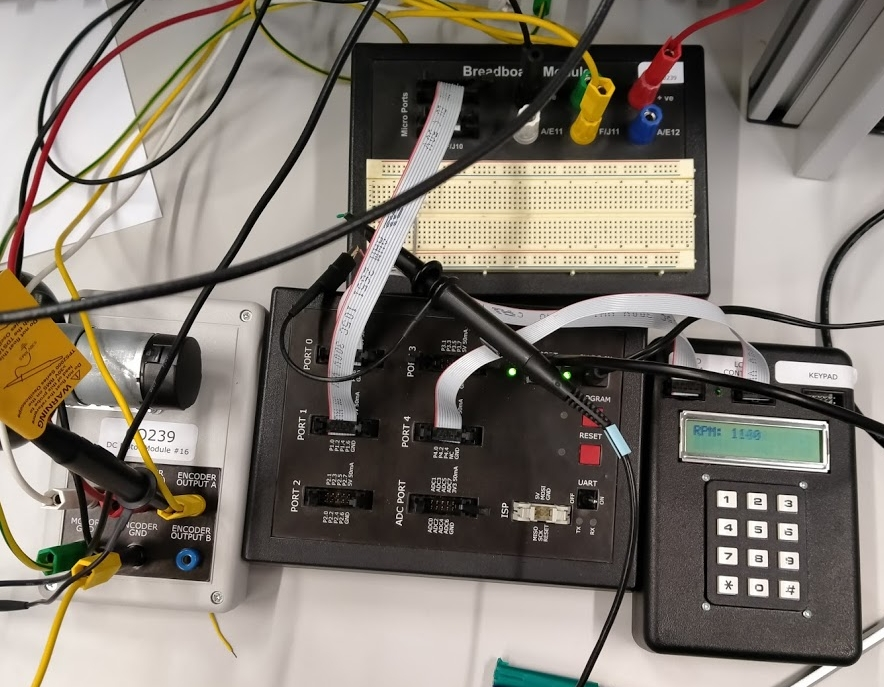
\includegraphics[width=0.5\textwidth]{inc/setup.jpg}
        \end{center}

        The software can then be configured to generate an interrupt from the external pulses, either on a single edge (left) resulting in a halved signal or on both the rising and falling edge. 
        This is configured with CAPMn.5\&4.

        \begin{center}
            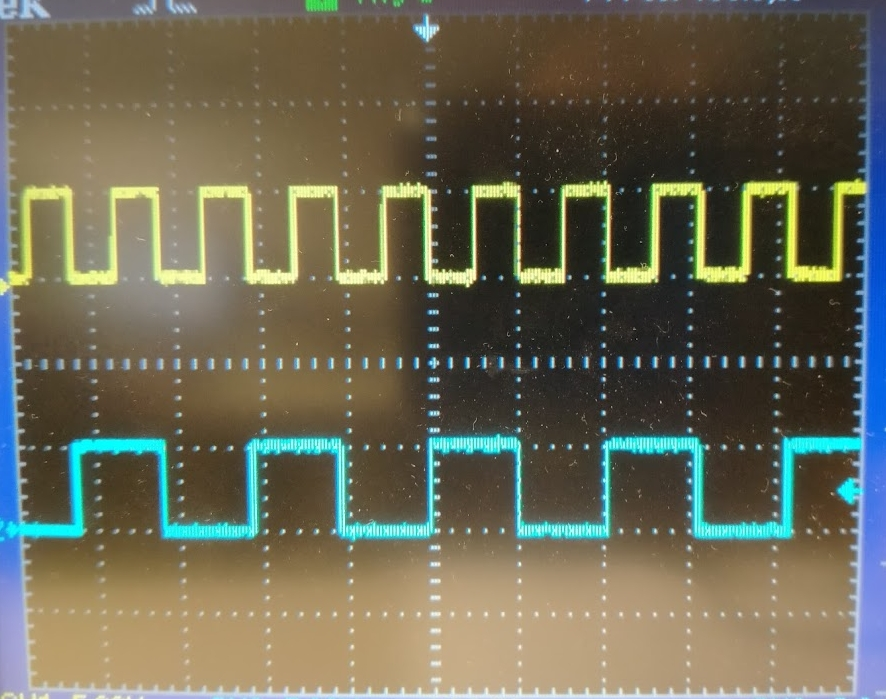
\includegraphics[width=0.3\textwidth]{inc/edge_single.jpg}
            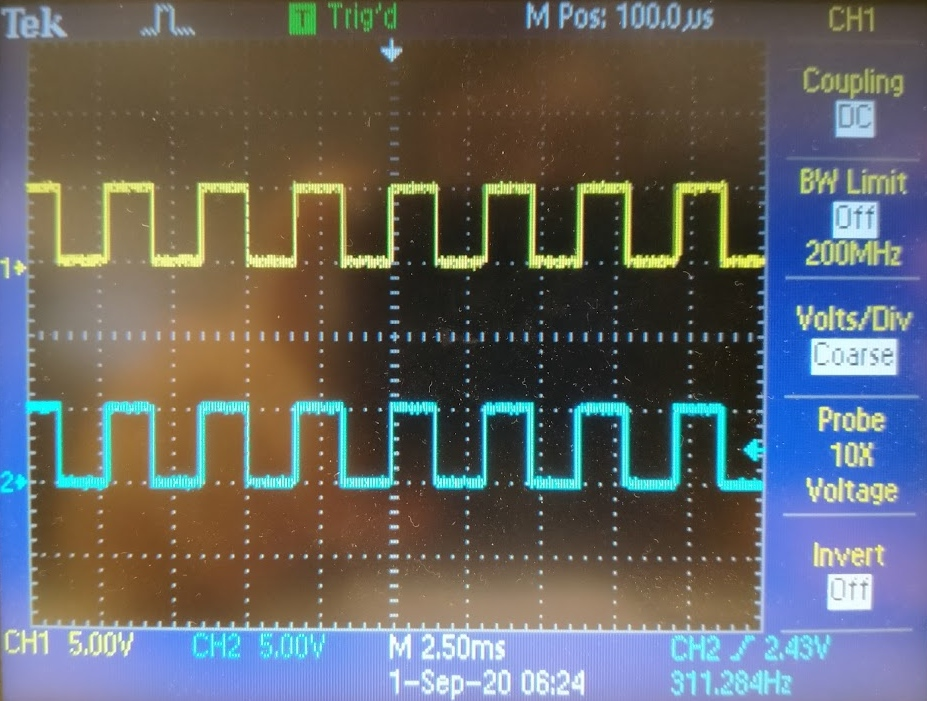
\includegraphics[width=0.3\textwidth]{inc/edged_double.jpg}
        \end{center}

        With the PCA timer enabled, the ISR can then use it to sample the timer between interrupts (ie pulses) and use the known values of the counter clock speed, encoder steps per revolution, and counter value to determine a revolutions per minute value to display to the LCD.

        \begin{center}
            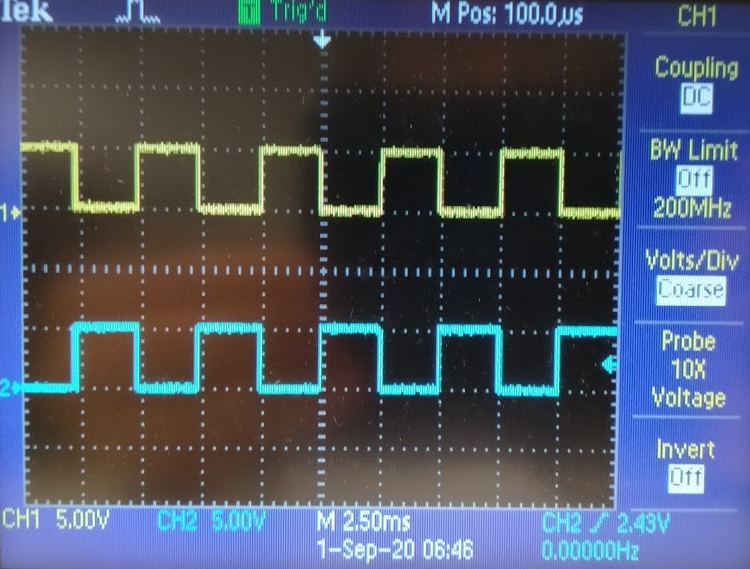
\includegraphics[width=0.3\textwidth]{inc/pulse_low.jpg}
            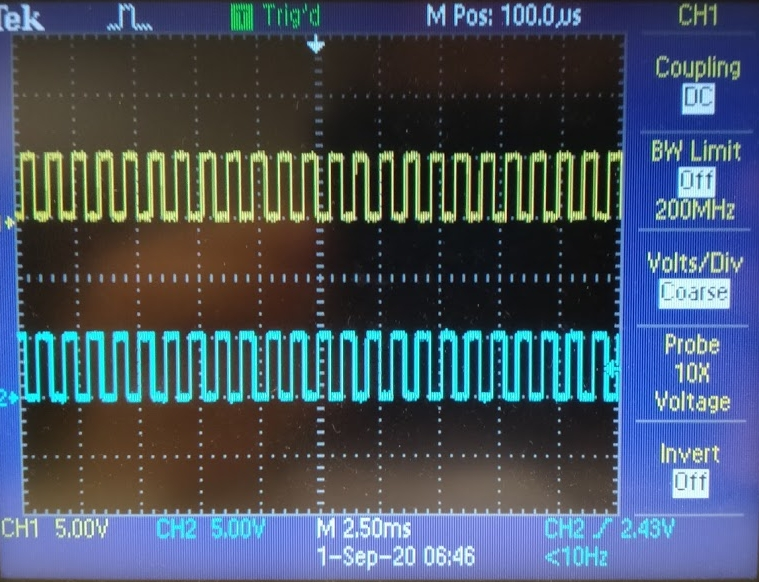
\includegraphics[width=0.3\textwidth]{inc/pulse_high.jpg}
            
            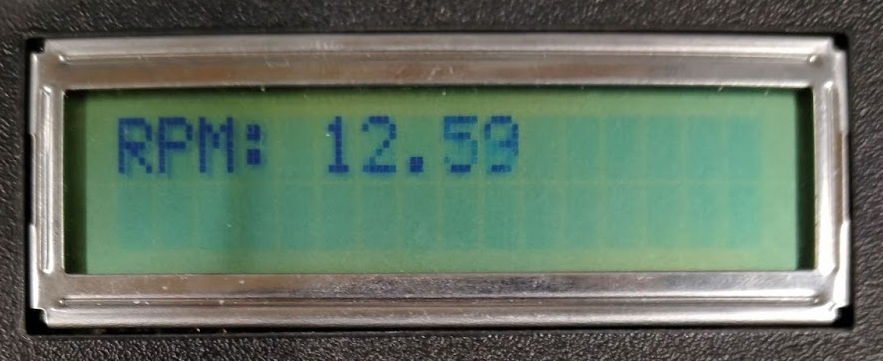
\includegraphics[width=0.3\textwidth]{inc/rpm_low.jpg}
            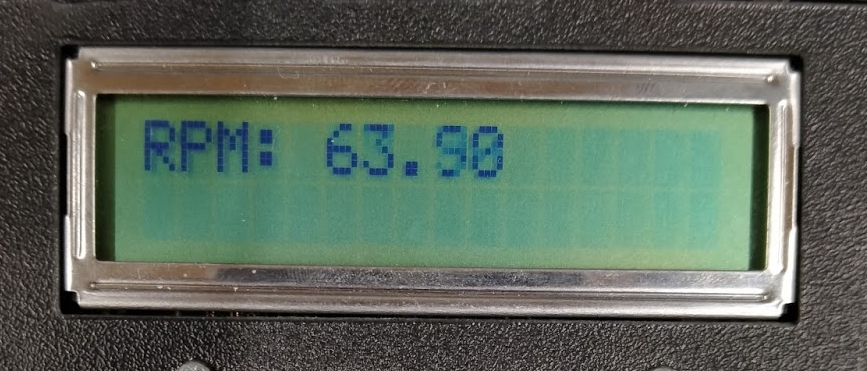
\includegraphics[width=0.3\textwidth]{inc/rpm_high.jpg}
        \end{center}


        \lstinputlisting[language=C, style=Cstyle]{inc/capture_intrpt.c}

        \subsection{Timer 0 and Calibrated Delay}
        \begin{center}
            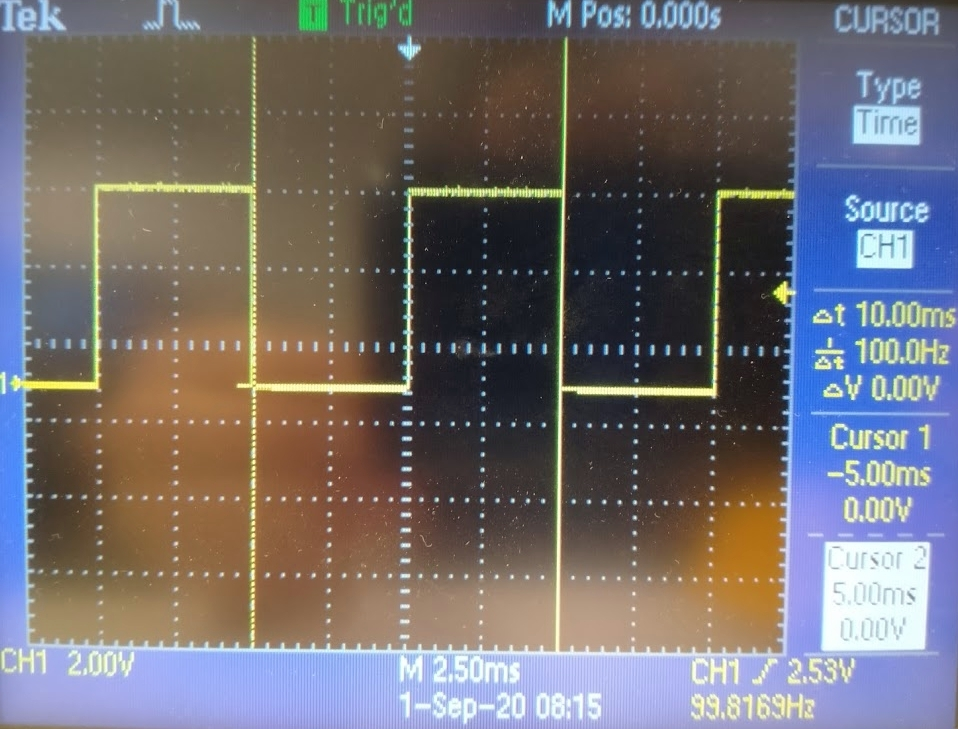
\includegraphics[width=0.42\textwidth]{inc/timer_10ms.jpg}
            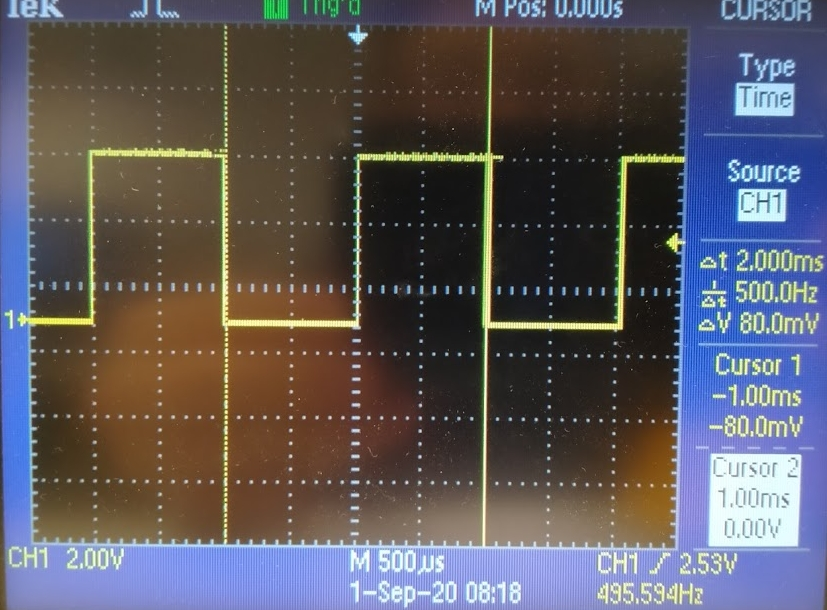
\includegraphics[width=0.42\textwidth]{inc/timer_2ms.jpg}
        \end{center}

        To improve upon the previous delay methods of just entering a set number of empty loops, the timer peripheral can be used to set an actual time value for the delay. Above shows the results of setting to 10mS and 2mS and below the is the implementation.

        To achieve a set time of a 1mS accurate the timer (in 8 bit mode) was preloaded at 6 $(2^8 - 6 = 250uS)$ assuming that the clock is at 1Mhz. I found that mine was in X2 mode and running at 2Mhz for had to count 8 overflows to get to 1mS.

        \lstinputlisting[language=C, style=Cstyle]{inc/delay_timer.c}
\section{Questions}
\begin{enumerate}
    \item \textit{\textbf{Given that you know the number of seconds in a minute; the number of counts occurring per second, the number of counts occurring per hole and the number of holes per revolution, find a formula for the RPM, the revolutions per minute.}}\\
    
    Known values are: 

    \textbf{480} holes per revolution of the encoder (double if using double edge trigger), PCA clock speed of \textbf{1Mhz} (1/6 of cpu clock by default) so 1uS increment time, and N as the increment count between interrupts. Therefore\dots

    $$RPM = \frac{60}{2{\cdot}480{\cdot}N{\cdot}1{\times}10^{-6}}$$
        
    \item \textit{\textbf{Can you make the timer more accurate? To the millisecond? To the microsecond? What are the advantages/disadvantages of doing this?}}\\
    
    The current implementation is currently millisecond accurate and relies and counting a set amount of timer overflows to achieve higher time intervals. To get a 'faster' delay function, say a single timer increment accurate the timer can be set into 16 bit mode and the timer duration is set by preloading the timer with a determined value and the overflow defined the end of the delay. Doing this increases the accuracy but in order to uncap the upper limit of $2^16 \times 1uS$ a second timer is needed. 
\end{enumerate}
\end{preview}
\end{document}